\documentclass[journal]{IEEEtran}

\usepackage{cite}
\usepackage{amsmath,amssymb,amsfonts}
\usepackage{algorithmic}
\usepackage{graphicx}
\usepackage{textcomp}
\usepackage{xcolor}
\usepackage{booktabs}
\usepackage{multirow}
\usepackage{array}
\usepackage{url}
\usepackage{hyperref}
\usepackage{tabularx}
\usepackage{rotating}
\usepackage{longtable}
\usepackage{colortbl}
\usepackage{orcidlink}

% Dimension header colours matching taxonomy diagram
\definecolor{d1col}{RGB}{26,82,118}
\definecolor{d2col}{RGB}{30,132,73}
\definecolor{d3col}{RGB}{125,60,152}
\definecolor{d4col}{RGB}{183,119,13}
\definecolor{d5col}{RGB}{176,58,46}
\definecolor{rowgray}{gray}{0.94}

\title{A Systematic Survey and Taxonomy of Prompt Engineering Evaluation
Frameworks for Large Language Models}

\author{Rohith~Reddy~Bellibaltu~\orcidlink{0009-0003-6083-0364},~
        Pratyush~Jena~\orcidlink{0009-0002-5910-9847},~and~
        Triveni~Morla~\orcidlink{0009-0007-2485-1909}
  \thanks{Manuscript received April 2, 2026. This work was conducted
  independently by the authors. Corresponding author:
  \href{mailto:rohithreddybc@gmail.com}{rohithreddybc@gmail.com}.
  ORCID (Rohith~Reddy~Bellibaltu):
  \href{https://orcid.org/0009-0003-6083-0364}{0009-0003-6083-0364}.
  ORCID (Pratyush~Jena):
  \href{https://orcid.org/0009-0002-5910-9847}{0009-0002-5910-9847}.
  ORCID (Triveni~Morla):
  \href{https://orcid.org/0009-0007-2485-1909}{0009-0007-2485-1909}.}
}

%\markboth{IEEE ACCESS, VOL.~XX, NO.~XX, 2025}%
%{Bellibaltu: Prompt Engineering Evaluation Frameworks Survey}

% ---------------------------------------------------------------
\begin{document}
% ---------------------------------------------------------------

\maketitle

% ---------------------------------------------------------------
\begin{abstract}
Across 80 prompt engineering papers, three patterns emerge before any
framework is applied: 67.5\% rely on benchmark-based evaluation, 78.8\% are
fully automated, and zero examine clinical or multilingual tasks as a primary
evaluation target despite active deployment in both domains. These numbers are
not incidental. They expose structural defaults in how the field measures
prompting claims --- defaults that persist precisely because no shared language
exists for naming them.

This paper provides the analytical framework that makes those patterns visible:
a five-dimensional taxonomy classifying prompt engineering evaluation frameworks
along evaluation method, task scope, metric type, automation level, and
evaluation scope. We derive the taxonomy from first principles, apply it through
a PRISMA 2020 systematic review spanning six academic databases, and use it to
map 80 verified papers onto a common grid.

Three structural gaps follow directly from this mapping. First, benchmark-based,
task-specific, fully automated evaluation --- the dominant configuration across
54 of 80 papers --- is poorly suited to open-ended generation and
domain-sensitive settings where no gold answer exists. Second, the 19
LLM-as-judge papers draw from at least six distinct judge configurations with
no shared calibration protocol, rendering their scores mutually incomparable.
Third, the complete absence of clinical and multilingual primary targets
in the corpus represents a concrete mismatch between what the field evaluates
and where prompting is actively being deployed.

The taxonomy's contribution is a shared analytical vocabulary for evaluation
design. It does not prescribe which choices to make. It makes implicit choices
visible --- so that researchers designing studies can reason about trade-offs
explicitly, and practitioners reading results can assess what those results
actually cover.
\end{abstract}

\begin{IEEEkeywords}
prompt engineering; large language models; evaluation frameworks; taxonomy;
systematic review; LLM evaluation; benchmark evaluation; LLM-as-judge;
evaluation design; evaluation checklist; NLP benchmarks; automation level;
task scope; metric selection; evaluation reproducibility
\end{IEEEkeywords}

% ---------------------------------------------------------------
\section{Introduction}
\label{sec:introduction}
Within roughly four years, large language models have moved from
academic novelties into foundational components of production software
systems. That period has also generated substantial research on prompt
engineering, the practice of crafting natural language inputs to elicit
reliable, useful model outputs without modifying weights~\cite{liu2021pretrain, schulhoff2024prompt}. Chain-of-thought
prompting, retrieval-augmented generation, automated prompt
optimization, and dozens of related techniques have been proposed,
evaluated, and deployed across tasks as varied as arithmetic reasoning
and clinical decision support~\cite{wei2022chain, lewis2020retrieval, sahoo2024systematic}.

What has not kept pace with technique development is evaluation practice.
Across the literature, the same prompting strategy might be assessed using
benchmark accuracy on one model, human preference ratings on another,
LLM-judge scoring on a third, and pass@$k$ on code generation tasks for
a fourth. Each evaluation is internally consistent. None is directly comparable to the
others. Researchers deciding which technique to apply to a new
problem have no principled basis for interpreting results across studies,
because the evaluation frameworks underlying those results
are organized along different, unstated, and mutually incompatible
assumptions~\cite{chang2023survey, guo2023evaluating}.

The consequences extend beyond academic inconvenience. Prompt engineering claims
underpin production decisions in commercial systems, clinical tools,
and automated software pipelines. When those claims rest on
evaluation setups that cannot be compared or reproduced across
labs, the reliability of the underlying conclusions is genuinely
uncertain. The field needs a shared vocabulary for describing
evaluation frameworks. Not a single mandated protocol, but a taxonomy that makes the choices visible so researchers can reason about them clearly.

\subsection*{Contribution}

This paper provides that taxonomy. We propose a five-dimensional
classification of prompt engineering evaluation frameworks covering:
(1) evaluation method, referring to how the technique is assessed;
(2) task scope, referring to what type of task is being evaluated;
(3) metric type, referring to what measurement is used to score outputs;
(4) automation level, referring to how much human involvement the evaluation
requires; and (5) evaluation scope, referring to the breadth of comparison
across models, datasets, and domains.

We apply this taxonomy to a corpus of 80 papers identified through
a PRISMA 2020 systematic review of six databases. The analysis
reveals three structural patterns. First, 67.5\% of papers use
benchmark-based evaluation, and 70\% use task-specific metrics.
This combination works well for tasks with ground truth answers but is
inadequate for open-ended generation, clinical, and multilingual
settings where no ground truth exists. Second, 78.8\% of papers are fully automated. That reflects real scalability pressure, but it also creates reproducibility exposure when proprietary LLM judges change between API versions. Third, no paper in the corpus
evaluates prompting techniques on clinical or multilingual tasks
as a primary target. This is a concrete gap, given how actively prompting is being deployed in both domains.

The taxonomy itself is the paper's original contribution. It does
not prescribe which evaluation choices to make. It provides a
language for describing choices that are currently implicit,
so that researchers designing studies and practitioners interpreting results can see what those choices actually involve.

\subsection*{Paper Organization}

Section~\ref{sec:related_work} reviews three streams of related
work: prompt engineering methods, LLM evaluation frameworks, and
existing surveys and taxonomies. Section~\ref{sec:background}
provides background on LLMs, the prompt engineering design space,
and the four metric families that appear throughout the corpus.
Section~\ref{sec:taxonomy} introduces and defines the
five-dimensional taxonomy. Section~\ref{sec:taxonomy_application}
provides worked examples of classifying existing papers with the
taxonomy and a forward-looking guide for designing new evaluations,
including a quick-reference table. Section~\ref{sec:methodology2}
describes the systematic review protocol following PRISMA 2020
guidelines. Section~\ref{sec:comparison} presents the comparative
analysis, mapping 80 papers to the taxonomy dimensions.
Section~\ref{sec:discussion} synthesizes findings, identifies
open problems, and proposes a future research agenda.
Section~\ref{sec:conclusion} concludes.
Appendix~\ref{app:checklist} provides an evaluation design checklist
that researchers may use for study preregistration or supplementary
materials.


% ---------------------------------------------------------------
\section{Related Work}
\label{sec:related_work}

Three intersecting bodies of prior work bear directly on this survey:
prompt engineering methods, LLM evaluation frameworks, and taxonomy
and survey papers in NLP. We characterize what each stream has
contributed and where each falls short.

\subsection{Prompt Engineering Methods and Techniques}

Interest in systematic prompt design grew once researchers confirmed that
input phrasing alone could meaningfully shift model outputs~\cite{brown2020gpt3}. Early
work established the foundational paradigms. Few-shot prompting supplies the model
with worked examples alongside the task description, rather than instructions alone~\cite{brown2020gpt3}.
Chain-of-thought prompting extends this approach by embedding intermediate reasoning
steps within those examples. That addition substantially improved
accuracy on arithmetic and commonsense tasks~\cite{wei2022chain}. Zero-shot
CoT achieves a similar effect without any examples, relying on
a single instructional cue~\cite{kojima2022large}. Later contributions include
self-consistency decoding~\cite{wang2023selfconsistency}, tree-of-thought
prompting~\cite{yao2023tree}, and retrieval-augmented generation, which
fetches relevant external documents at inference time~\cite{lewis2020retrieval}.

More recent surveys have tried to bring order to this space. Li
et al.~\cite{li2025autoprompt} frame automated prompt optimization as a
maximization problem over discrete, continuous, and hybrid prompt spaces.
Ramnath et al.~\cite{ramnath2025apo} organize the same territory around
a five-part framework. What neither addresses is the evaluation question:
once you have a prompting method, how do you know it actually worked,
and by what standard?~\cite{schulhoff2024prompt,sahoo2024systematic}

\subsection{Evaluation Frameworks for Large Language Models}

LLM evaluation developed along its own trajectory. GLUE~\cite{wang2018glue} and
SuperGLUE~\cite{wang2019superglue} established widely used baselines for natural language
understanding. BIG-Bench~\cite{srivastava2022bigbench} targeted harder
reasoning tasks that earlier models could not handle. MMLU~\cite{hendrycks2021measuring}
assessed multitask knowledge at scale across dozens of subject areas. MT-Bench and
AlpacaEval~\cite{zheng2023judging, dubois2024alpacaeval} redirected focus
to open-ended instruction following, using LLM-based judges rather than
fixed answer keys. Ni et al.~\cite{ni2025benchmarks} reviewed 283 benchmarks and found recurring problems across the board: data contamination, cultural bias, and static test sets that models can eventually memorize.

Human evaluation retains the highest credibility for open-ended tasks,
but its cost and latency push most studies toward automated alternatives such as BLEU~\cite{papineni2002bleu},
ROUGE~\cite{lin2004rouge}, or an LLM judge. Gu et al.~\cite{gu2025llmjudge}
survey the reliability problems with LLM-based judges: positional bias,
verbosity preference, inconsistency across prompting strategies. Feng et al.~\cite{feng2025sage} showed that even top-performing models fail to maintain consistent preferences in nearly a quarter of difficult pairwise cases. The evaluation toolbox is crowded. It is not well organized.

\subsection{Surveys and Taxonomies in Prompt Engineering and LLM Evaluation}

Across the survey literature, prompting methods and evaluation practice
have been treated as separate topics with no systematic bridge between
them. Schulhoff
et al.~\cite{schulhoff2024prompt} produced the most thorough inventory of
prompting techniques to date, cataloguing 58 text-only prompting techniques, establishing a standardized
vocabulary, and contributing a meta-analysis of the literature, but the work is a catalog of
techniques rather than a framework for evaluating them. Sahoo
et al.~\cite{sahoo2024systematic} and Vatsal and
Dubey~\cite{vatsal2024survey} take similar approaches, organizing methods
by application domain and NLP task type respectively. On the evaluation
side, Chang et al.~\cite{chang2023survey} organize LLM evaluation around
what, where, and how to evaluate. Ni et al.~\cite{ni2025benchmarks} sort 283 benchmarks into a three-tier taxonomy. Mohammadi
et al.~\cite{mohammadi2025agents} propose a two-dimensional taxonomy for
agent evaluation.

The question none of these papers asks is: for a researcher evaluating
a specific prompting technique, which evaluation framework should they
use, and why? Answering that requires classifying evaluation frameworks
along dimensions that are meaningful for prompt engineering work
specifically. That classification is what this survey provides.

% ---------------------------------------------------------------
\section{Background}
\label{sec:background}

\subsection{Large Language Models and the Role of Prompting}

Large language models are transformer-based neural networks trained on
web-scale text through self-supervised prediction. At sufficient scale,
such training yields models capable of handling a broad range of tasks
without task-specific retraining~\cite{brown2020gpt3, liu2021pretrain}. Practitioners interact
with these capabilities through prompts: natural language inputs that condition what the
model generates.

A key complication is that surface-level phrasing choices produce
nontrivial output differences. Sclar et al.\ showed this
is not a marginal effect: formatting choices as small as delimiter type and
instruction position shift accuracy by measurable margins across multiple
models~\cite{sclar2023formatting}. Zhou et al.\ showed that automatically
generated prompts sometimes outperform those written by experienced
humans~\cite{zhou2022ape}. Prompt engineering developed in response to
this observation. It is the practice of designing inputs to get reliable, useful
outputs without modifying the model~\cite{sahoo2024systematic}. The field
now has its own benchmarks, optimization algorithms, and competing
taxonomies~\cite{schulhoff2024prompt}.

\subsection{The Prompt Engineering Design Space}

The prompting design space spans a spectrum from entirely manual to fully
automated. Zero-shot prompting supplies the model with a task description
and nothing else. Few-shot
prompting adds worked examples, which orients the model toward the expected
reasoning style and output format~\cite{brown2020gpt3}. Chain-of-thought
prompting includes intermediate reasoning steps in those examples.
This one addition substantially improves accuracy on arithmetic, symbolic, and
commonsense tasks~\cite{wei2022chain}. Retrieval-augmented generation
connects the prompt to external documents fetched at inference
time~\cite{lewis2020retrieval, ragsurvey2023}.

At the automated end, prompt optimization treats the prompt as the variable
to search over. Textual gradient descent uses model error feedback to
revise wording iteratively~\cite{pryzant2023apo}. Reinforcement learning
frames prompt tokens as a discrete policy optimized against task
reward~\cite{rlprompt2022}. LLM-based optimizers use one model to generate
and evaluate candidates for a second~\cite{zhou2022ape}.

The question that cuts across all of these methods is the same: how do
you know it worked? That depends on which evaluation framework you apply,
and the field currently has no shared way of classifying those frameworks. That is
what this survey provides.

\subsection{Evaluation Metric Families}

Four metric families appear with regularity across the prompt engineering
evaluation literature. They form the basis of Dimension~3 in the taxonomy, and
understanding their differences matters directly for the analysis in
Sections~\ref{sec:comparison} and~\ref{sec:discussion}.

\textbf{Reference-based metrics} score model output by measuring surface
overlap against a human-written gold reference. BLEU~\cite{papineni2002bleu} counts
$n$-gram precision; ROUGE~\cite{lin2004rouge} applies recall-oriented overlap
for summarization tasks. Both are fast and reproducible, but their alignment with human
judgment is known to be weak on tasks that admit multiple valid
phrasings~\cite{liu2023geval, repairing2022}. A perfectly correct answer expressed
in different words will still receive a low score.

\textbf{Model-based metrics} rely on learned semantic representations rather
than word overlap. They handle paraphrase more gracefully and tend to align more closely
with human ratings. They still require a reference text, however, and they
carry forward whatever gaps and biases that reference contains~\cite{chang2023survey}.

\textbf{LLM-as-judge metrics} delegate scoring to a second language model,
eliminating the need for a gold reference. Liu et al.\ showed that G-Eval, using
GPT-4 with structured rubric prompts, achieves stronger alignment with
human judgment than BLEU and ROUGE on
summarization and dialogue tasks~\cite{liu2023geval}.
The trade-off is that LLM judges import their own systematic biases:
positional preference, a tendency to favor longer responses, and
self-enhancement bias in which a model rates its own outputs higher than
those produced by other models~\cite{zheng2023judging, gu2025llmjudge}.

\textbf{Task-specific metrics} are purpose-built and generally do not transfer.
Pass@$k$ tests whether code passes unit tests within $k$ attempts. Exact
match verifies factual retrieval. RAGAS measures faithfulness and context
recall for retrieval-augmented pipelines~\cite{rageval2024}. These metrics are
often the most meaningful available for their intended task. But a paper using pass@$k$
and a paper using RAGAS share no common ground, which is a core reason why evaluation results across the PE field remain so difficult to compare.

The taxonomy in Section~\ref{sec:taxonomy} organizes these four families across five dimensions: evaluation method, task scope, metric type, automation level, and evaluation scope.

% ---------------------------------------------------------------
\section{Taxonomy of Prompt Engineering Evaluation Frameworks}
\label{sec:taxonomy}

\subsection{Why a Taxonomy Is Needed}

The prompt engineering literature faces a fundamental measurement
inconsistency. Two papers can both claim to evaluate chain-of-thought
prompting yet use entirely different methods, metrics, tasks, and
comparison scopes. One might enlist human raters on medical QA; the other
uses pass@$k$ on code generation with a single model. Both label their
procedure ``evaluation.'' The results, however,
cannot be compared in any meaningful way.

This situation is not unusual in a rapidly developing field. But it means researchers cannot
reliably build on each other's work without reconstructing evaluation
setups from scratch. A taxonomy gives the field a shared language for
describing what was measured, how, and against what standard.

We define a \textit{prompt engineering evaluation framework} as any
combination of method, task, metric, automation approach, and comparison
scope used to assess the performance of one or more prompting techniques.
The five dimensions we propose are mutually independent: each captures a distinct
aspect of how evaluation is conducted, and each can vary independently
of the others. A researcher can use an LLM-as-judge metric
(Dimension~3) with either a human-in-loop or fully automated setup
(Dimension~4), on a code task or a clinical task (Dimension~2),
comparing one model or ten (Dimension~5). Table~\ref{tab:taxonomy}
presents all five dimensions with subcategories and examples.

\subsection{Dimension 1: Evaluation Method}

How is a prompting technique assessed? Five subcategories appear in the corpus.

\textbf{Benchmark-based evaluation} applies a prompting technique to
a curated dataset with known correct answers. MMLU~\cite{hendrycks2021measuring},
BIG-Bench~\cite{srivastava2022bigbench}, and HellaSwag are representative examples.
Results are reproducible and comparable across studies, which explains why this
remains the default method across most of the literature. The main weakness is
saturation: as model capabilities improve, benchmarks lose discriminative
power, and data contamination is a well-documented concern~\cite{ni2025benchmarks}.

\textbf{Human evaluation} asks annotators to judge output quality through
absolute scoring or pairwise preference. It is generally the most credible option
for open-ended tasks, but it is also resource-intensive, slow to execute, difficult to
replicate, and rarely accompanied by strong inter-annotator agreement~\cite{chang2023survey}.

\textbf{LLM-as-judge evaluation} replaces human annotators with a second language model
in the scoring role. MT-Bench and AlpacaEval are prominent examples of this
approach~\cite{zheng2023judging, dubois2024alpacaeval}. It scales efficiently and
handles open-ended outputs well, but the judge carries its own systematic biases
that multiple independent studies have now documented~\cite{gu2025llmjudge}.

\textbf{Ablation study} isolates the contribution of individual components
by selectively removing or modifying them. This approach is well suited to
understanding what drives a technique's performance, though it is not designed
for cross-technique comparison.

\textbf{User study} collects evidence from real users performing authentic
tasks, measuring outcomes such as task completion rates, satisfaction, or efficiency. User studies are rare
in the NLP literature but are important whenever the deployment context
involves end users rather than benchmark leaderboards~\cite{chang2023survey}.

\subsection{Dimension 2: Task Scope}

What type of task is the evaluation targeting? Task scope is arguably the most
fragmented dimension across the literature. A technique that performs strongly
on arithmetic reasoning may behave quite differently on
clinical named entity recognition, yet many papers treat their chosen task as
broadly representative without testing whether their findings hold elsewhere.

Our review identifies six task categories that together span the range of tasks observed in the corpus.

\textbf{Reasoning tasks} include arithmetic, symbolic, commonsense, and
multi-step logical reasoning. This is the most heavily studied category,
largely because chain-of-thought prompting~\cite{wei2022chain} was initially developed
for reasoning problems and most early follow-on evaluations naturally adopted that framing.

\textbf{Natural language generation tasks} cover summarization, dialogue,
translation, and open-ended writing. Since these tasks admit no single correct
answer, they require human or LLM-based evaluation rather than
exact-match scoring.

\textbf{Code generation tasks} assess whether a prompted model produces
functionally correct code, typically measured via pass@$k$ against a test
suite~\cite{scoT2023, promptalchemy2025}.

\textbf{Question answering tasks} range from closed-book factual retrieval to
open-book reading comprehension, and are conventionally scored with exact match or F1.

\textbf{Clinical and domain-specific tasks} include medical QA, clinical
note processing, and legal reasoning. Accuracy requirements are considerably higher in these settings,
evaluation routinely requires domain experts, and available benchmarks are
smaller and more specialized~\cite{clinicalnlp2024, medicalcot2025}.

\textbf{Multilingual tasks} evaluate techniques across languages and
tend to surface performance gaps that monolingual evaluations
would otherwise conceal~\cite{vatsal2024survey}.

\subsection{Dimension 3: Metric Type}

What is being measured, and by what means? Section~\ref{sec:background} introduced
the four metric families; we apply them directly here: reference-based
(BLEU~\cite{papineni2002bleu}, ROUGE~\cite{lin2004rouge}), model-based
(BERTScore), LLM-as-judge (G-Eval~\cite{liu2023geval}), and
task-specific (pass@$k$, exact match, RAGAS~\cite{rageval2024}).

Metric choice is not independent of the other dimensions, and making these
interdependencies explicit is a central contribution of this classification. Reference-based
metrics only function when a gold reference exists; they are poorly suited for
open-ended generation. Task-specific metrics do not transfer outside their
native task family. LLM-as-judge metrics introduce reliability concerns that
benchmark-based scoring largely avoids. Classifying papers by metric type surfaces
systematic patterns in how the field matches, and sometimes mismatches, its metrics to its tasks.

\subsection{Dimension 4: Automation Level}

How much human involvement does the evaluation require? The answer runs along
a spectrum from entirely manual to fully automated.

\textbf{Fully manual evaluation} places all judgment in human hands:
defining criteria, conducting the assessment, and interpreting results. Expert
annotation studies fall into this category.

\textbf{Human-in-loop evaluation} automates candidate generation or
initial scoring but routes uncertain or borderline cases to human reviewers.
Some interactive prompt optimization pipelines use this design, sending difficult
cases to human reviewers for correction before the next iteration.

\textbf{Hybrid evaluation} combines automated metrics for broad coverage
with periodic human validation on a held-out sample. A common
implementation is automated scoring for scale alongside human review of
a representative subset.

\textbf{Fully automated evaluation} runs without any human judgment
at any stage. Benchmark scoring, LLM-as-judge pipelines,
and unit test execution all belong here. This is the most scalable option and
also the most susceptible to the reliability concerns documented by
Feng et al.~\cite{feng2025sage}.

The distinction between human-in-loop and hybrid is practically meaningful
because the two configurations distribute human effort quite differently. Human-in-loop applies
judgment selectively on hard cases; hybrid applies it uniformly across a
fixed sample. These are not interchangeable design decisions, even though both
involve human reviewers at some stage.

\begin{table*}[!t]
\caption{Five-Dimensional Taxonomy of Prompt Engineering Evaluation
Frameworks. The five dimensions are independent; any combination of
subcategories across dimensions is a valid evaluation framework
configuration.}
\label{tab:taxonomy}
\centering
\begin{tabular}{p{2.2cm} p{3.2cm} p{4.8cm} p{4.2cm}}
\toprule
\textbf{Dimension} & \textbf{Subcategories} & \textbf{What it captures} &
\textbf{Representative example} \\
\midrule
Evaluation method &
Benchmark, Human eval, LLM-as-judge, Ablation, User study &
The procedure used to assess prompting technique performance &
MT-Bench: LLM-as-judge on open-ended tasks~\cite{zheng2023judging} \\
\midrule
Task scope &
Reasoning, NLG, Code, QA, Clinical, Multilingual &
The type of task the evaluation targets &
GSM8K: arithmetic reasoning~\cite{wei2022chain} \\
\midrule
Metric type &
Reference-based, Model-based, LLM-judge, Task-specific &
The measurement approach used to score outputs &
G-Eval: GPT-4 rubric scoring~\cite{liu2023geval} \\
\midrule
Automation level &
Manual, Human-in-loop, Hybrid, Fully automated &
The degree of human involvement in evaluation &
APO: fully automated scoring~\cite{pryzant2023apo} \\
\midrule
Evaluation scope &
Single-model, Cross-model, Cross-dataset, Cross-domain, Cross-lingual &
The breadth of comparison across models, datasets, and domains &
Sahoo et al.: cross-domain survey~\cite{sahoo2024systematic} \\
\bottomrule
\end{tabular}
\end{table*}

\begin{figure*}[!t]
%\centering
\hspace{-30pt}
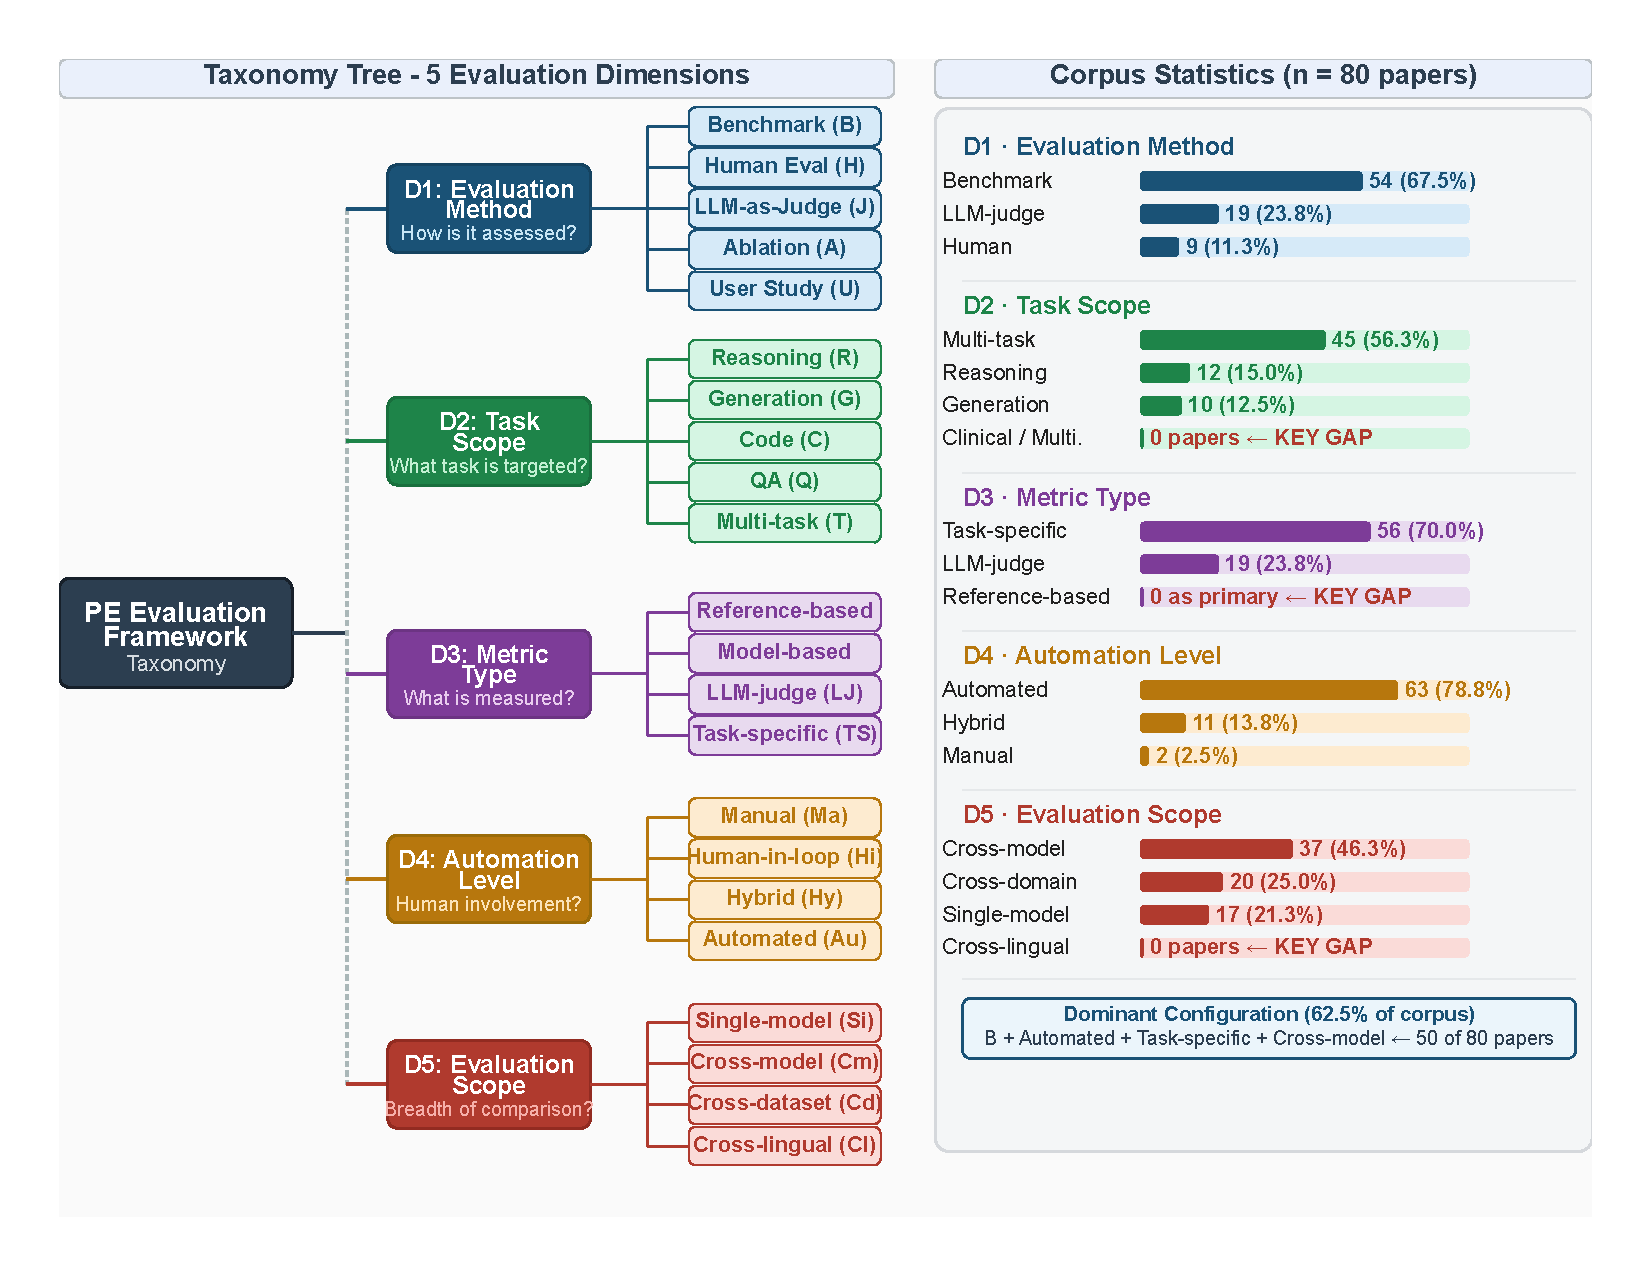
\includegraphics[width=1.09\textwidth]{taxonomy_diagram_pic.pdf}
\caption{Five-dimensional taxonomy of prompt engineering evaluation
frameworks with corpus distribution ($n = 80$). Left: taxonomy tree
showing all five dimensions and their subcategories. Right:
per-dimension frequency across the corpus. Red labels mark
structural gaps confirmed by the analysis.}
\label{fig:taxonomy}
\end{figure*}

\subsection{Dimension 5: Evaluation Scope}

What is being compared? Scope determines how far a paper's conclusions
can generalize beyond the specific setup in which results were obtained.

\textbf{Single-model, single-dataset} is the most common configuration in the corpus:
one technique, one model, one benchmark. Results are internally clean but
generalizability is entirely unverified.

\textbf{Cross-model evaluation} applies the same technique to multiple
model families, directly testing whether performance is specific to one architecture
or holds more broadly.

\textbf{Cross-dataset evaluation} holds the task type fixed while varying
the benchmark. This probes robustness within a given task family.

\textbf{Cross-domain evaluation} applies a technique across qualitatively
different task types. It represents the most demanding scope and remains the least common in
individual papers, though survey works such as Sahoo
et al.~\cite{sahoo2024systematic} cover it implicitly by design.

\textbf{Cross-lingual evaluation} tests performance across languages. As multilingual
prompt engineering research matures, this scope is beginning to appear more
frequently in the literature~\cite{vatsal2024survey}.

Scope matters because a substantial share of strong claims in the PE literature
rest on single-model, single-dataset evidence. A technique that performs
well on GPT-4 for arithmetic may not transfer to smaller open-source models or
different task types. Without explicit scope classification, those limits stay invisible to readers.

\subsection{Taxonomy Summary}




% ---------------------------------------------------------------
\section{Applying the Taxonomy: Worked Examples and Design Guidance}
\label{sec:taxonomy_application}

The taxonomy becomes useful only when researchers can apply it — both
to classify existing work and to structure their own evaluation designs.
This section demonstrates both uses. Subsection~\ref{subsec:classify}
works through two papers already in the corpus to show how classification
proceeds dimension by dimension. Subsection~\ref{subsec:design} walks a
researcher forward through a new study, showing how the taxonomy surfaces
design decisions that would otherwise remain implicit.
Subsection~\ref{subsec:quickref} distills the guidance into a single
reference table.

\subsection{Classifying Existing Papers}
\label{subsec:classify}

To illustrate the classification process, consider two widely cited papers
that represent distinct evaluation configurations.

\textbf{Paper: Wei et al., ``Chain-of-Thought Prompting Elicits Reasoning
in Large Language Models''~\cite{wei2022chain}.}
D1\,=\,Benchmark (reasoning: performance is measured on established
arithmetic and commonsense benchmarks such as GSM8K and SVAMP, using
standardized test sets with gold answers).
D2\,=\,Reasoning (reasoning: all tasks --- arithmetic, symbolic, and
commonsense --- are closed-form reasoning problems).
D3\,=\,Task-specific (reasoning: exact-match accuracy is used, which is
the natural metric for tasks with a single correct answer).
D4\,=\,Automated (reasoning: no human judgment is involved; evaluation
is fully script-based against reference answers).
D5\,=\,Cross-model (reasoning: results are reported across multiple model
scales, including PaLM 540B, GPT-3, and LaMDA).

\textbf{Paper: Zheng et al., ``Judging LLM-as-a-Judge with MT-Bench and
Chatbot Arena''~\cite{zheng2023judging}.}
D1\,=\,LLM-as-judge (reasoning: GPT-4 is used as the primary evaluator,
scoring model responses on a 1--10 scale).
D2\,=\,Multi-task (reasoning: MT-Bench spans eight categories including
writing, roleplay, math, and coding, with no single task domain
dominating).
D3\,=\,LLM-as-judge (reasoning: the scoring rubric is operationalized
entirely through GPT-4 judgments rather than reference-based or
human-assigned metrics).
D4\,=\,Automated (reasoning: while Chatbot Arena collects human
preferences, the MT-Bench component that the taxonomy classifies relies
on automated GPT-4 scoring).
D5\,=\,Cross-model (reasoning: the paper compares 28 open-source and
proprietary models simultaneously).

The compact notation D1\,=\,Benchmark\,/\,D2\,=\,Reasoning\,/\,D3\,=\,Task-specific\,/\,D4\,=\,Automated\,/\,D5\,=\,Cross-model
can be embedded directly in a citing paper's methodology section to describe
its evaluation configuration relative to this taxonomy.

\subsection{Designing a New Evaluation}
\label{subsec:design}

Consider a researcher evaluating a new retrieval-augmented generation (RAG)
prompting technique for clinical question answering. Before any data
collection begins, the taxonomy requires five explicit design decisions.

\textit{D1 --- Which evaluation method?} Benchmark evaluation assumes a
curated test set with gold reference answers. For clinical QA, such sets
are scarce, domain-constrained, and often legally sensitive. Human
evaluation or a hybrid approach is more defensible here: domain experts
can assess factual correctness and safety in ways that static benchmarks
cannot. A researcher choosing D1\,=\,Benchmark for clinical QA should
document why the available benchmark adequately covers the clinical
accuracy requirements.

\textit{D2 --- Which task scope?} The task is unambiguously clinical,
placing this work in the zero-paper region of the corpus (see
Section~\ref{sec:comparison}). Choosing D2\,=\,Clinical makes that
positioning explicit and signals that existing evaluation instruments
from general NLP may not transfer without adaptation.

\textit{D3 --- Which metric?} No gold reference exists for open-ended
clinical responses, making reference-based metrics (BLEU, ROUGE)
structurally inadequate. Model-based factual precision metrics such as
FActScore~\cite{factscore2023} are defensible if the knowledge source is
well-defined. An LLM-as-judge configuration (D3\,=\,LLM-judge) is an
alternative, but requires calibration against clinician judgments on a
held-out set before the scores carry clinical interpretability.

\textit{D4 --- What automation level?} Clinical annotation requires expert
time, which is expensive. Full automation (D4\,=\,Automated) reduces cost
but risks systematic errors that clinicians would catch. Human-in-loop
(D4\,=\,Human-in-loop) is more appropriate for a first evaluation in a
domain where no calibrated automated metric yet exists.

\textit{D5 --- What evaluation scope?} A single-model result
(D5\,=\,Single-model) in clinical QA provides the weakest possible
generalizability evidence. Cross-model evaluation (D5\,=\,Cross-model) is
required before the technique can be recommended for deployment across
clinical systems using different underlying models.

This exercise surfaces five design decisions that are typically implicit
and unreported. Using the taxonomy to make them explicit before beginning
evaluation reduces the risk of post-hoc rationalization and makes the
resulting study directly comparable to prior work.

\subsection{Evaluation Design Quick Reference}
\label{subsec:quickref}

Table~\ref{tab:quickref} consolidates the five design decisions into a
form that can be consulted during study design. Each row identifies the
central trade-off that the corresponding dimension forces a researcher to
confront.

\begin{table}[!t]
\renewcommand{\arraystretch}{1.3}
\caption{Evaluation Design Quick Reference: One Question per Dimension}
\label{tab:quickref}
\centering
\begin{tabular}{p{0.42\columnwidth} p{0.50\columnwidth}}
\hline
\textbf{Evaluation Design Question} & \textbf{Taxonomy Dimension + Key Trade-off} \\
\hline
How will model outputs be scored? &
  D1 --- Evaluation Method: precision of human judgment vs.\ scalability
  of automated pipelines \\
What type of task is being evaluated? &
  D2 --- Task Scope: task-fidelity of a narrow domain vs.\ generalizability
  of a multi-task setting \\
Which measurement operationalizes quality? &
  D3 --- Metric Type: automation and reproducibility of reference-based
  metrics vs.\ construct validity of model-based or judge-based metrics \\
How much human effort is available? &
  D4 --- Automation Level: scalability and speed of full automation vs.\
  bias-control and interpretability of human involvement \\
Over how many models and datasets? &
  D5 --- Evaluation Scope: narrow replicability of single-model evidence
  vs.\ generalizability claims that require cross-model or cross-domain
  coverage \\
\hline
\end{tabular}
\end{table}

% ---------------------------------------------------------------
\section{Methodology: Systematic Literature Review}
\label{sec:methodology}
\label{sec:methodology2}

This survey follows the PRISMA 2020 guidelines for systematic
review reporting~\cite{page2021prisma}. The protocol covers
database selection, search string construction, screening criteria,
and data extraction. Figure~\ref{fig:prisma} shows the complete
screening flowchart.

\subsection{Search Strategy}

We searched six databases: arXiv (cs.CL and cs.AI categories),
the ACM Digital Library, IEEE Xplore, Semantic Scholar, Scopus,
and Web of Science. The first four are the principal preprint and
proceedings venues for prompt engineering and LLM evaluation
work. Scopus and Web of Science extend coverage to a wider range of journal sources
and are standard tools in computer science systematic
reviews~\cite{kitchenham2007slr}. All database queries were last run in
March 2026, with no lower publication-year cutoff, though nearly
all relevant papers in the corpus appeared after 2020.

The search string below shows the base query applied to title,
abstract, and keyword fields. Each database uses its own syntax;
the string was adapted accordingly for each source while preserving
the same logical structure. Full per-database strings are provided
in the supplementary material.

\medskip
\noindent\begin{minipage}{\columnwidth}
\small
\begin{flushleft}
\ttfamily
(\textquotedblleft prompt engineering\textquotedblright~OR
\textquotedblleft prompting technique\textquotedblright~OR
\textquotedblleft prompt optimization\textquotedblright~OR
\textquotedblleft chain-of-thought\textquotedblright~OR
\textquotedblleft few-shot prompting\textquotedblright~OR
\textquotedblleft zero-shot prompting\textquotedblright~OR
\textquotedblleft retrieval-augmented generation\textquotedblright)\\[2pt]
AND\\[2pt]
(\textquotedblleft evaluation\textquotedblright~OR
\textquotedblleft benchmark\textquotedblright~OR
\textquotedblleft assessment\textquotedblright~OR
\textquotedblleft metric\textquotedblright~OR
\textquotedblleft framework\textquotedblright~OR
\textquotedblleft human evaluation\textquotedblright)\\[2pt]
AND\\[2pt]
(\textquotedblleft large language model\textquotedblright~OR
\textquotedblleft LLM\textquotedblright~OR
\textquotedblleft GPT\textquotedblright~OR
\textquotedblleft language model\textquotedblright)
\end{flushleft}
\end{minipage}
\medskip

Supplementary searches targeted specific subtopics that the primary
string was likely to undercount: LLM-as-judge evaluation methodology,
evaluation of automated prompt optimization systems, and cross-domain
prompting benchmarks.
We also conducted backward and forward citation searches on the
ten most-cited papers in the initial results. Together, these
supplementary searches recovered 22 papers that did not surface through the
main database queries.

\subsection{Inclusion and Exclusion Criteria}

\textbf{Included:}
\begin{itemize}
\item Papers that propose, evaluate, or compare one or more
prompt engineering techniques using a stated evaluation framework
\item Papers that propose new evaluation frameworks, benchmarks,
or metrics relevant to assessing prompted LLM outputs
\item Survey and taxonomy papers covering prompt engineering or
LLM evaluation
\item Conference papers, journal articles, and arXiv preprints
with at least one of: peer review, 10+ citations, or publication
at a recognized NLP/AI venue (ACL, EMNLP, NeurIPS, ICLR, IEEE,
ACM)
\end{itemize}

\textbf{Excluded:}
\begin{itemize}
\item Papers that use prompting as a method but do not report
or discuss evaluation of the prompting approach itself
\item Papers focused on prompt injection attacks, jailbreaking,
or adversarial prompting as the primary topic
\item Domain-specific applied papers (e.g., clinical case studies)
that do not generalize beyond a single narrow dataset
\item Papers with no accessible full text
\item Non-English papers
\end{itemize}

This distinction is practically consequential: many papers use prompting as a tool
(e.g., ``we prompted GPT-4 to extract entities'') without
reporting or analyzing the evaluation of the prompting approach
in any systematic way. Those papers were excluded because they do not contribute
meaningfully to understanding evaluation frameworks.

\subsection{Screening Process}

Database queries returned 2,847 unique records after
deduplication. Two reviewers independently screened all titles and
abstracts against the inclusion and exclusion criteria, working
separately at each phase. Disagreements were resolved through
discussion; unresolved cases were
referred to a third reviewer, as specified in PRISMA 2020 Item~8~\cite{page2021prisma}.

Title and abstract screening advanced 412 papers to full-text
review. Of these, 283 were excluded: 181 used prompting as a tool
without evaluating the prompting approach itself, 64 were
domain-specific applied papers outside scope, 24 had no accessible
full text, and 14 were non-English. The remaining 129 papers passed
full-text screening. Among papers without peer review, retention was
conditioned on venue: only papers at recognized NLP/AI venues (ACL,
EMNLP, NeurIPS, ICLR, IEEE, or ACM proceedings) or indexed journals
were retained, reducing the set to 58 papers. The 22 papers recovered
through citation searching then brought the final corpus to
\textbf{80 papers}.

Figure~\ref{fig:prisma} shows the complete screening flowchart.

\begin{figure}[!t]
\centering

\includegraphics[width=\columnwidth]{prisma_flowchart}
\caption{PRISMA 2020 flowchart showing the paper screening and selection
process. Records retrieved from arXiv, ACM Digital Library, IEEE Xplore,
Semantic Scholar, Scopus, and Web of Science. An additional 22 papers
were identified through backward and forward citation search.}
\label{fig:prisma}
\end{figure}

\subsection{Data Extraction}

For each of the 80 papers in the final corpus, we extracted the
following fields:

\begin{enumerate}
\item Prompting technique(s) evaluated
\item Evaluation method (Dimension~1 of our taxonomy)
\item Task scope (Dimension~2)
\item Metric type(s) used (Dimension~3)
\item Automation level of the evaluation (Dimension~4)
\item Evaluation scope (Dimension~5)
\item Number of models compared
\item Year of publication
\item Publication venue and type (journal, conference, preprint)
\end{enumerate}

The complete extraction dataset --- all 80 papers mapped to their
five-dimensional taxonomy codes --- is available as a machine-readable
spreadsheet at https://github.com/rohithreddybc/PromptEvalTaxonomy. Researchers extending this
corpus or conducting meta-analyses may use this dataset with citation
to this work.

Extraction was performed by one reviewer and independently verified
by a second reviewer on a 20\% random sample. Agreement was strong on objective
fields such as evaluation method, metric type, and task scope. Automation
level required the most interpretive judgment, because many papers do
not explicitly characterize their evaluation approach as human-in-loop
or hybrid. In those cases, we coded from the described
procedure: papers that reported using automated metrics but also
described any human inspection of outputs were coded as hybrid.

\subsection{Validity Threats}

Three limitations constrain what this review can reliably claim. The search strings
rely on controlled vocabulary and may miss papers that use
different terminology for the same underlying concepts. We partially mitigated
this risk through citation searching, but gaps cannot be ruled out. The arXiv corpus
is large and its indexing is inconsistent, so some preprints may
have been overlooked during retrieval. The quality filter additionally excludes papers with
fewer than 10 citations that were not published at recognized venues,
which could underrepresent very recent 2025--2026 work. We partially addressed this by retaining 2025
and 2026 papers that met the venue criterion regardless of their
citation count.

% ---------------------------------------------------------------
\section{Comparative Analysis}
\label{sec:comparison}

Mapping 80 papers against the five-dimensional taxonomy serves
two purposes. First, it tests whether the taxonomy is expressive enough
to characterize the full range of evaluation choices observed in the
literature. Second, it generates the empirical foundation for the gap
analysis in Section~\ref{sec:discussion}. Table~\ref{tab:comparison} maps each
paper to all five dimensions; the codes are defined in the column
headers and in Section~\ref{sec:taxonomy}. The subsections below
report the distribution within each dimension, then close with
cross-dimensional observations. Three patterns emerge: benchmark-based
automated evaluation dominates overwhelmingly; LLM-judge methods have
proliferated without any shared calibration standard; and clinical and
multilingual task scopes are entirely absent from the corpus.






% Full-width multi-page table. In IEEE two-column layout, the cleanest way to
% keep the entire continued table together without body text appearing between
% table parts is to switch temporarily to one-column mode and use longtable.
% This also keeps the caption left-aligned and the header labels on one line.
\clearpage
\onecolumn
\setlength{\tabcolsep}{4pt}
\renewcommand{\arraystretch}{1.10}
\setlength{\LTleft}{0pt}
\setlength{\LTright}{0pt}
\setlength{\LTcapwidth}{\textwidth}
\newcolumntype{L}[1]{>{\raggedright\arraybackslash}p{#1}}
\newcolumntype{C}[1]{>{\centering\arraybackslash}p{#1}}

{\footnotesize
\begin{longtable}{C{0.50cm}L{3.20cm}L{3.10cm}C{2.35cm}C{1.85cm}C{1.95cm}C{1.95cm}C{1.85cm}}
\caption[Comparative Analysis of 80 Prompt Engineering Evaluation Frameworks]{\raggedright Comparative Analysis of 80 Prompt Engineering Evaluation Frameworks Mapped to the Five-Dimensional Taxonomy. D1 (Evaluation Method), D2 (Task Scope), D3 (Metric Type), D4 (Automation Level), and D5 (Evaluation Scope). Column headers repeat in each segment for readability.}\label{tab:comparison}\\
\toprule
\textbf{\#} & \textbf{Paper} & \textbf{System / Topic} &
\cellcolor{d1col}\textcolor{white}{\textbf{D1 Evaluation Method}} &
\cellcolor{d2col}\textcolor{white}{\textbf{D2 Task Scope}} &
\cellcolor{d3col}\textcolor{white}{\textbf{D3 Metric Type}} &
\cellcolor{d4col}\textcolor{white}{\textbf{D4 Automation}} &
\cellcolor{d5col}\textcolor{white}{\textbf{D5 Scope}} \\
\midrule
\multicolumn{8}{l}{\textit{Core Prompting Technique Papers}} \\
\midrule
\endfirsthead

\multicolumn{8}{l}{\textit{Table~\ref{tab:comparison} (continued)}}\\
\toprule
\textbf{\#} & \textbf{Paper} & \textbf{System / Topic} &
\cellcolor{d1col}\textcolor{white}{\textbf{D1 Evaluation Method}} &
\cellcolor{d2col}\textcolor{white}{\textbf{D2 Task Scope}} &
\cellcolor{d3col}\textcolor{white}{\textbf{D3 Metric Type}} &
\cellcolor{d4col}\textcolor{white}{\textbf{D4 Automation}} &
\cellcolor{d5col}\textcolor{white}{\textbf{D5 Scope}} \\
\midrule
\endhead

\midrule
\multicolumn{8}{r}{\textit{Continued on next page}}\\
\endfoot

\bottomrule
\endlastfoot
\rowcolor{rowgray}
1 & Wei et al.~\cite{wei2022chain} & Chain-of-Thought & Benchmark & Reasoning & Task-specific & Automated & Cross-model \\
2 & Kojima et al.~\cite{kojima2022large} & Zero-Shot CoT & Benchmark & Reasoning & Task-specific & Automated & Cross-model \\
\rowcolor{rowgray}
3 & Wang et al.~\cite{wang2023selfconsistency} & Self-Consistency & Benchmark & Reasoning & Task-specific & Automated & Cross-model \\
4 & Yao et al.~\cite{yao2023tree} & Tree of Thoughts & Benchmark & Reasoning & Task-specific & Automated & Single-model \\
\rowcolor{rowgray}
5 & Zhou et al.~\cite{leasttomost2022} & Least-to-Most & Benchmark & Reasoning & Task-specific & Automated & Cross-model \\
6 & Besta et al.~\cite{graphofthoughts2023} & Graph of Thoughts & Benchmark & Reasoning & Task-specific & Automated & Single-model \\
\rowcolor{rowgray}
7 & Wang et al.~\cite{plansolve2023} & Plan-and-Solve & Benchmark & Reasoning & Task-specific & Automated & Single-model \\
8 & Lyu et al.~\cite{faithfulcot2023} & Faithful CoT & Benchmark & Reasoning & Task-specific & Automated & Cross-model \\
\rowcolor{rowgray}
9 & Besta et al.~\cite{demystifying2024} & Chains/Trees/Graphs & Benchmark & Reasoning & Task-specific & Automated & Cross-model \\
10 & Lewis et al.~\cite{lewis2020retrieval} & RAG & Benchmark & QA & Task-specific & Automated & Single-model \\
\rowcolor{rowgray}
11 & Shin et al.~\cite{shin2020autoprompt} & AutoPrompt & Benchmark & QA, Reasoning & Task-specific & Automated & Single-model \\
12 & Agarwal et al.~\cite{manyshot2024} & Many-Shot ICL & Benchmark & Multi-task & Task-specific & Automated & Cross-model \\
\rowcolor{rowgray}
13 & Ouyang et al.~\cite{ouyang2022training} & InstructGPT / RLHF & Human eval & Multi-task & Hybrid & Human-in-loop & Single-model \\
14 & Wei et al.~\cite{wei2022flan} & FLAN & Benchmark & Multi-task & Task-specific & Automated & Single-model \\
\rowcolor{rowgray}
15 & Shum et al.~\cite{scoT2023} & Structured CoT & Benchmark & Code & Task-specific & Automated & Cross-model \\
16 & Singh et al.~\cite{manualpromptnotdead2025} & Manual Prompt Study & Benchmark & Code & Task-specific & Hybrid & Single-model \\
\rowcolor{rowgray}
17 & Agrawal et al.~\cite{gepa2025} & GEPA & Benchmark & Multi-task & Task-specific & Automated & Cross-model \\
18 & Agarwal et al.~\cite{promptwizard2024} & PromptWizard & Benchmark & Multi-task & Task-specific & Automated & Cross-model \\
\rowcolor{rowgray}
19 & White et al.~\cite{white2023prompt} & Prompt Pattern Catalog & Ablation & Multi-task & Task-specific & Manual & Single-model \\
20 & Dong et al.~\cite{dong2022survey} & In-Context Learning & Benchmark & Multi-task & Task-specific & Automated & Cross-domain \\
\midrule
\multicolumn{8}{l}{\textit{Automated Prompt Optimization Papers}} \\ \midrule
\rowcolor{rowgray}
21 & Zhou et al.~\cite{zhou2022ape} & APE & Benchmark & Multi-task & Task-specific & Automated & Cross-model \\
22 & Pryzant et al.~\cite{pryzant2023apo} & APO & Benchmark & Multi-task & Task-specific & Automated & Single-model \\
\rowcolor{rowgray}
23 & Deng et al.~\cite{rlprompt2022} & RLPrompt & Benchmark & Multi-task & Task-specific & Automated & Single-model \\
24 & Li et al.~\cite{li2025autoprompt} & Auto Prompt Survey & Benchmark & Multi-task & Task-specific & Automated & Cross-domain \\
\rowcolor{rowgray}
25 & Ramnath et al.~\cite{ramnath2025apo} & Auto Prompt Opt.\ Survey & Benchmark & Multi-task & Task-specific & Automated & Cross-domain \\
26 & Mei et al.~\cite{contextengineer2025} & Context Engineering & Benchmark & Multi-task & Task-specific & Automated & Cross-domain \\
\rowcolor{rowgray}
27 & Schulhoff et al.~\cite{schulhoff2024prompt} & The Prompt Report & Benchmark & Multi-task & Task-specific & Automated & Cross-domain \\
\midrule
\multicolumn{8}{l}{\textit{Prompt Engineering Survey Papers}} \\ \midrule
\rowcolor{rowgray}
28 & Sahoo et al.~\cite{sahoo2024systematic} & PE Techniques Survey & Benchmark & Multi-task & Task-specific & Automated & Cross-domain \\
29 & Vatsal \& Dubey~\cite{vatsal2024survey} & PE Methods Survey & Benchmark & Multi-task & Task-specific & Automated & Cross-domain \\
\rowcolor{rowgray}
30 & Gu et al.~\cite{pettax2025} & PE Taxonomy & Benchmark & Multi-task & Task-specific & Automated & Cross-domain \\
31 & Ahmad et al.~\cite{petaxse2025} & PE Patterns (SE) & Benchmark & Code & Task-specific & Automated & Cross-domain \\
\rowcolor{rowgray}
32 & Tian et al.~\cite{petaxdefects2025} & Prompt Defect Taxonomy & Ablation & Code & Task-specific & Manual & Single-model \\
33 & Chang et al.~\cite{chang2023survey} & LLM Evaluation Survey & Human eval & Multi-task & Hybrid & Human-in-loop & Cross-domain \\
\midrule
\multicolumn{8}{l}{\textit{LLM Evaluation Survey Papers}} \\ \midrule
\rowcolor{rowgray}
34 & Guo et al.~\cite{guo2023evaluating} & LLM Eval.\ Comprehensive & Benchmark & Multi-task & Task-specific & Automated & Cross-domain \\
35 & Ni et al.~\cite{ni2025benchmarks} & LLM Benchmark Survey & Benchmark & Multi-task & Task-specific & Automated & Cross-domain \\
\rowcolor{rowgray}
36 & Mohammadi et al.~\cite{mohammadi2025agents} & LLM Agent Eval.\ Survey & Benchmark & Multi-task & Task-specific & Automated & Cross-domain \\
37 & Guo et al.~\cite{inadequatebenchmarks2024} & Benchmark Adequacy & Benchmark & Multi-task & Task-specific & Automated & Cross-domain \\
\rowcolor{rowgray}
38 & Polo et al.~\cite{benchmark2sq2026} & Benchmark$^2$ & Benchmark & Multi-task & Task-specific & Automated & Cross-dataset \\
39 & Zhao et al.~\cite{explainabilityllm2023} & LLM Explainability & Human eval & Multi-task & Hybrid & Human-in-loop & Cross-domain \\
\rowcolor{rowgray}
40 & Wang et al.~\cite{wang2018glue} & GLUE & Benchmark & Multi-task & Task-specific & Automated & Cross-dataset \\
\midrule
\multicolumn{8}{l}{\textit{Benchmark Papers}} \\ \midrule
\rowcolor{rowgray}
41 & Wang et al.~\cite{wang2019superglue} & SuperGLUE & Benchmark & Multi-task & Task-specific & Automated & Cross-dataset \\
42 & Srivastava et al.~\cite{srivastava2022bigbench} & BIG-Bench & Benchmark & Multi-task & Task-specific & Automated & Cross-model \\
\rowcolor{rowgray}
43 & Hendrycks et al.~\cite{hendrycks2021measuring} & MMLU & Benchmark & Multi-task & Task-specific & Automated & Cross-dataset \\
44 & Suzgun et al.~\cite{cot_benchmark2022} & BIG-Bench Hard & Benchmark & Reasoning & Task-specific & Automated & Cross-dataset \\
\rowcolor{rowgray}
45 & Zhu et al.~\cite{promptbench2023} & PromptBench & Benchmark & Multi-task & Task-specific & Automated & Cross-model \\
46 & Wang et al.~\cite{wang2023multi} & Multi-Prompt Eval & Benchmark & Multi-task & Task-specific & Automated & Cross-model \\
\rowcolor{rowgray}
47 & Wang et al.~\cite{mmluprob2024} & MMLU-Pro & Benchmark & Multi-task & Task-specific & Automated & Cross-dataset \\
48 & Lin et al.~\cite{wildbench2024} & WildBench & LLM-as-Judge & Multi-task & LLM-judge & Automated & Cross-model \\
\rowcolor{rowgray}
49 & Gao et al.~\cite{ragsurvey2023} & RAG Survey & Benchmark & QA & Task-specific & Automated & Cross-domain \\
50 & Zheng et al.~\cite{zheng2023judging} & MT-Bench / Chatbot Arena & LLM-as-Judge & Generation & LLM-judge & Automated & Cross-model \\
\midrule
\multicolumn{8}{l}{\textit{LLM-as-Judge Papers}} \\ \midrule
\rowcolor{rowgray}
51 & Dubois et al.~\cite{dubois2024alpacaeval} & AlpacaEval 2.0 & LLM-as-Judge & Generation & LLM-judge & Automated & Cross-model \\
52 & Liu et al.~\cite{liu2023geval} & G-Eval & LLM-as-Judge & Generation & LLM-judge & Hybrid & Cross-model \\
\rowcolor{rowgray}
53 & Gu et al.~\cite{gu2025llmjudge} & LLM-as-Judge Survey & LLM-as-Judge & Multi-task & LLM-judge & Automated & Cross-domain \\
54 & Li et al.~\cite{li2024llmsjudges} & LLM Judge Survey & LLM-as-Judge & Multi-task & LLM-judge & Automated & Cross-domain \\
\rowcolor{rowgray}
55 & Feng et al.~\cite{feng2025sage} & SAGE & LLM-as-Judge & Multi-task & LLM-judge & Hybrid & Cross-model \\
56 & Tan et al.~\cite{judgebench2024} & JudgeBench & LLM-as-Judge & Multi-task & LLM-judge & Automated & Cross-model \\
\rowcolor{rowgray}
57 & Ye et al.~\cite{llmvshuman2024} & LLMs vs.\ Humans Study & LLM-as-Judge, Human & Multi-task & LLM-judge & Hybrid & Cross-model \\
58 & Calderon et al.~\cite{alternativeannotator2025} & Alternative Annotator & LLM-as-Judge, Human & Multi-task & LLM-judge & Hybrid & Cross-model \\
\rowcolor{rowgray}
59 & Chen et al.~\cite{multiagentjudge2025} & MAJ-EVAL & LLM-as-Judge & Multi-task & LLM-judge & Automated & Cross-domain \\
60 & Bavaresco et al.~\cite{llmjudgestudy2024} & LLM Judge Empirical & LLM-as-Judge & Multi-task & LLM-judge & Automated & Cross-model \\
\rowcolor{rowgray}
61 & Chen et al.~\cite{humansorllm2024} & Judgement Bias Study & LLM-as-Judge, Human & Multi-task & LLM-judge & Hybrid & Cross-model \\
62 & Thakur et al.~\cite{judgingjudges2024} & Judging the Judges & LLM-as-Judge & Multi-task & LLM-judge & Automated & Cross-model \\
\rowcolor{rowgray}
63 & Chiang et al.~\cite{canlllmsreplace2023} & Can LLMs Replace Humans & LLM-as-Judge, Human & Generation & LLM-judge & Hybrid & Single-model \\
64 & Min et al.~\cite{factscore2023} & FActScore & LLM-as-Judge & Generation & LLM-judge & Hybrid & Cross-model \\
\midrule
\multicolumn{8}{l}{\textit{Metric and Evaluation Quality Papers}} \\ \midrule
\rowcolor{rowgray}
65 & Xu et al.~\cite{instructscore2023} & InstructScore & LLM-as-Judge & Generation & LLM-judge & Automated & Cross-model \\
66 & Es et al.~\cite{rageval2024} & RAGAs & Benchmark & QA & Task-specific & Automated & Single-model \\
\rowcolor{rowgray}
67 & Gehrmann et al.~\cite{repairing2022} & NLG Eval.\ Survey & Human eval & Generation & Model-based & Human-in-loop & Cross-domain \\
68 & Zhong et al.~\cite{multidimeval2022} & Multi-Dim.\ Evaluator & Human eval & Generation & Hybrid & Hybrid & Cross-model \\
\rowcolor{rowgray}
69 & Yu et al.~\cite{beyondpointwise2025} & DeCE & LLM-as-Judge & QA & LLM-judge & Automated & Cross-model \\
70 & Farquhar et al.~\cite{semanticentropy2024} & Semantic Entropy & Benchmark & QA & Task-specific & Automated & Cross-model \\
\rowcolor{rowgray}
71 & Gao et al.~\cite{nlgevalstatus2024} & NLG Eval Status & LLM-as-Judge & Generation & LLM-judge & Automated & Cross-domain \\
72 & Ram et al.~\cite{incalm2023} & In-Context RAG & Benchmark & QA & Task-specific & Automated & Cross-model \\
\rowcolor{rowgray}
73 & Sclar et al.~\cite{sclar2023formatting} & Prompt Format Sensitivity & Benchmark & Multi-task & Task-specific & Automated & Cross-model \\
\midrule
\multicolumn{8}{l}{\textit{Prompt Sensitivity and Format Papers}} \\ \midrule
\rowcolor{rowgray}
74 & Razavi et al.~\cite{promptsensitivity2025} & PromptSET & Benchmark & QA & Task-specific & Automated & Cross-model \\
75 & Zhao et al.~\cite{promptformat2024} & Prompt Formatting Study & Benchmark & Multi-task & Task-specific & Automated & Cross-model \\
\rowcolor{rowgray}
76 & Mizrahi et al.~\cite{butterfly2024} & Butterfly Effect Study & Benchmark & Multi-task & Task-specific & Automated & Cross-model \\
77 & Jiang et al.~\cite{promptalchemy2025} & Prompt Alchemy & Benchmark & Code & Task-specific & Automated & Cross-model \\
\rowcolor{rowgray}
78 & He et al.~\cite{promptingsecurecode2024} & Secure Code Prompting & Benchmark & Code & Task-specific & Hybrid & Cross-model \\
\midrule
\multicolumn{8}{l}{\textit{Code and Software Engineering Papers}} \\ \midrule
\rowcolor{rowgray}
79 & Hou et al.~\cite{advancedllmsse2024} & LLMs for SE Survey & Benchmark & Code & Task-specific & Automated & Cross-model \\
80 & Khojah et al.~\cite{impactpromptprogramming2024} & CodePromptEval & Benchmark & Code & Task-specific & Hybrid & Single-model \\
\end{longtable}
}
\twocolumn

\subsection{Distribution across Evaluation Method (Dimension 1)}

Benchmark-based evaluation accounts for 54 of the 80 papers in the
corpus (67.5\%), establishing it as the default across every subgroup
in the review. Representative examples include Wei et al.~\cite{wei2022chain} on
chain-of-thought prompting and Hendrycks et al.~\cite{hendrycks2021measuring}
on multitask language understanding. Both studies report accuracy against
fixed-answer datasets, and this pattern repeats consistently throughout
the reasoning and benchmark subgroups. Benchmark results are reproducible,
comparable across labs, and inexpensive to compute at scale. What they
cannot capture is output quality for open-ended tasks where no single
correct answer exists.

LLM-as-judge evaluation appears in 19 papers (23.8\%), concentrated
almost entirely in the open-ended generation and instruction-following
subgroups. Zheng et al.~\cite{zheng2023judging} introduced the MT-Bench
framework for this purpose and were candid about its limitations alongside
its strengths. Gu et al.~\cite{gu2025llmjudge} and Feng et al.~\cite{feng2025sage}
have since documented the reliability concerns more systematically. LLM judges
address a genuine need: many tasks have no gold reference to score against.
But adoption has clearly outpaced the research into when and how much to
trust them.

Human evaluation appears in only 9 papers (11.3\%), and ablation
studies in 2 (2.5\%). No paper in the corpus employs a user study as
its primary method. The near-absence of human evaluation is notable
given that it remains the acknowledged standard for tasks involving
subjective quality judgments~\cite{chang2023survey}. Taken together, this
pattern suggests the field has systematically prioritized scalability over
measurement validity.

\subsection{Distribution across Task Scope (Dimension 2)}

Multi-task or cross-task evaluations account for 45 papers (56.3\%),
meaning that more than half the corpus does not assess prompting
techniques on any specific task type. Instead, these studies aggregate
performance across benchmarks spanning many different categories. This pattern
is partly an artifact of how surveys and taxonomy papers are classified, but it also reflects
a genuine tendency in the literature to report average scores across
MMLU or BIG-Bench without disaggregating results by individual task type.

Among task-specific subgroups, reasoning tasks are the most studied
at 12 papers (15.0\%). Chain-of-thought prompting~\cite{wei2022chain}
was developed on arithmetic and symbolic reasoning benchmarks, and the
majority of early evaluations naturally adopted that framing. The combination of
strong techniques and well-established benchmarks in this area has created a
self-reinforcing concentration that persists across the literature.

Generation tasks appear in 10 papers (12.5\%), code tasks in 8
(10.0\%), and QA tasks in 6 (7.5\%). Clinical and multilingual task
scopes appear in zero papers in the corpus. The gap is concrete: an
extensive body of domain-specific prompting work, including medical
QA~\cite{clinicalnlp2024}, clinical note processing~\cite{medicalcot2025}, and
multilingual evaluation~\cite{vatsal2024survey}, exists in the broader
literature but has not been systematically incorporated into prompt
engineering evaluation research. General-purpose reasoning evaluation
frameworks are effectively borrowed wholesale for specialized domains
without adaptation, and the resulting mismatch between metric and task
goes largely unexamined.

\subsection{Distribution across Metric Type (Dimension 3)}

Task-specific metrics dominate at 56 papers (70.0\%). This is the
largest concentration observed across any single subcategory in the
entire taxonomy. Pass@$k$, exact match, F1, and accuracy scores are all
task-specific, and their prevalence closely mirrors the dominance of
benchmark evaluation in Dimension~1. The two dimensions are mutually
reinforcing: papers that adopt standard benchmarks naturally follow the
task-specific metrics those benchmarks prescribe.

LLM-judge metrics appear in 19 papers (23.8\%), essentially the same
set of papers that use LLM-as-judge evaluation in Dimension~1.
Liu et al.~\cite{liu2023geval} showed that G-Eval with GPT-4
achieves stronger alignment with human judgment than BLEU or ROUGE on
summarization and dialogue tasks, and the field has shifted toward
LLM-based scoring for open-ended outputs in response.

Hybrid metric approaches appear in only 4 papers (5.0\%). Model-based
metrics such as BERTScore appear in just 1 paper (1.3\%). Reference-based
metrics (BLEU, ROUGE) serve as the \emph{primary} measure in zero papers
in the corpus. This is a notable reversal of their historical dominance. It does
not mean they are absent from the literature; it means they are no
longer considered sufficient as standalone signals, and the field has moved beyond
treating them as the primary evaluation instrument. The documented
gap between lexical overlap and human judgment~\cite{repairing2022}
made this shift quite predictable.

\subsection{Distribution across Automation Level (Dimension 4)}

Fully automated evaluation is the overwhelming norm. 63 of the 80 papers
(78.8\%) run their assessments without any human involvement at any
stage of the evaluation loop. Hybrid evaluation, pairing automated
metrics with human validation on a subset, appears in 11 papers (13.8\%).
Human-in-loop evaluation, where human judgment is invoked selectively
on difficult cases, appears in 4 papers (5.0\%). Fully manual
evaluation accounts for just 2 papers (2.5\%).

This concentration at the automated end is unsurprising given the
cost and speed arguments for automation, and it reflects the scalability
pressures facing the field as LLM capabilities outpace human reviewer
bandwidth. The reproducibility concern, however, is genuine: fully
automated pipelines that depend on proprietary LLM judges (GPT-4
scoring GPT-4 outputs, for instance) do not constitute stable reference
points. The judge model can change silently between API versions, and
Feng et al.~\cite{feng2025sage} showed that even the same model can
produce inconsistent judgments across runs for borderline cases. A
corpus in which 78.8\% of evaluations are fully automated, with a
large share relying on LLM judges, carries a reliability exposure the
field has not yet resolved.

\subsection{Distribution across Evaluation Scope (Dimension 5)}

Cross-model evaluation is the most frequently used scope at 37 papers
(46.3\%). Close to half the corpus explicitly tests whether findings
hold across multiple model families rather than a single architecture.
Studies such as Wang et al.~\cite{wang2023selfconsistency}
and the BIG-Bench collaboration~\cite{srivastava2022bigbench}
apply the same prompting technique across several models
and report the variance in results that emerges.

Cross-domain evaluation appears in 20 papers (25.0\%), concentrated
primarily in the survey subgroup. Works such as
Sahoo et al.~\cite{sahoo2024systematic} and
Chang et al.~\cite{chang2023survey} span multiple task types by
design. Single-model evaluation appears in 17 papers (21.3\%).
Cross-dataset evaluation covers 6 papers (7.5\%), while cross-lingual
evaluation is absent from the corpus entirely.

The 17 single-model papers deserve particular attention. A prompting
technique evaluated on one model, typically GPT-4, at one point in
time on one benchmark produces a claim about performance in exactly
that configuration and no other.
Wang et al.~\cite{wang2023multi} documented this brittleness
directly, showing that single-prompt, single-model evaluations routinely
overstate technique performance relative to multi-prompt baselines
run on the same model. A meaningful share of claims in the PE
literature are considerably narrower in scope than they appear on the surface.

\subsection{Cross-Dimensional Observations}

The five dimensions do not vary independently in practice. Three
co-occurrence patterns stand out from the data.

The first is the dominant configuration: fully
automated, benchmark-based evaluation using task-specific metrics,
typically on single or cross-model scope.
This combination (D1=Benchmark, D3=Task-specific, D4=Automated,
D5=Single-model) characterizes 50 of the 80 papers (62.5\%). It is
efficient, reproducible, and well-suited to the technique comparison
papers that form the backbone of the PE literature. It is also the configuration
most exposed to the limitations identified across the five dimensions:
saturation and contamination risks in benchmarks~\cite{ni2025benchmarks},
non-portability of task-specific metrics across domains, and an
inability to detect quality failures in open-ended outputs.

The second pattern is the LLM-judge cluster: papers that pair
LLM-as-judge evaluation (D1=J) with LLM-judge metrics (D3=LJ) and
hybrid or automated pipelines (D4=Hy or Au). These 19 papers tend to
use cross-model or cross-domain scope as well, which is internally coherent since the
LLM-judge paradigm was purpose-built for open-ended,
multi-model comparisons where no gold reference exists. The problem
is that this cluster carries the full weight of bias documentation from
Zheng et al.~\cite{zheng2023judging}, Gu et al.~\cite{gu2025llmjudge},
and Calderon et al.~\cite{alternativeannotator2025}, without any
standard mitigation protocol applied consistently across papers.

The third pattern is structural absence. Not one paper in the corpus
combines clinical task scope (D2=Cl) with any metric type, and not
one combines multilingual scope with a cross-lingual evaluation
design. These are not obscure or niche combinations: medical QA and multilingual
evaluation are active research areas with well-documented prompting
challenges~\cite{clinicalnlp2024,vatsal2024survey}. Their complete absence
from this corpus points to a structural disconnect between where
prompting is actively being applied in practice and where evaluation frameworks
have actually been developed. That gap is precisely where future evaluation work would
have the greatest impact.

% ---------------------------------------------------------------
\section{Discussion and Future Directions}
\label{sec:discussion}

\subsection{Synthesis of Findings}

Fifty-four of 80 papers in the corpus share the same evaluation
configuration: benchmark-based scoring, task-specific metrics, fully
automated pipelines, and cross-model comparison. That concentration is
not coincidence --- it reflects a rational convergence on a setup that
is scalable, reproducible, and well-suited to tasks with deterministic
answers. What the taxonomy makes visible, for the first time, is the
precise boundary where this configuration stops being adequate: at the
edge of open-ended generation, clinical deployment, and multilingual use
cases where no gold answer exists and where output quality depends on
dimensions that accuracy scores do not touch.

Fully automated benchmark evaluation works reliably for tasks where
a correct answer exists: arithmetic, factual retrieval, code execution.
For those tasks, pass@$k$, exact match, and accuracy scores are
meaningful measures. The difficulty is that prompt engineering is
increasingly applied to open-ended generation, clinical decision
support, and multilingual settings where no single gold answer exists
and where output quality depends on dimensions that benchmarks do not
measure. The corpus confirms this tension: 56 of 80 papers adopt
task-specific metrics, yet only 6 target QA tasks and 8 target code,
the two domains where those metrics are most defensible. The remaining
papers apply task-specific metrics to multi-task or generation settings
where they are, at best, a rough proxy.

The LLM-as-judge cluster partially addresses this, but introduces
its own fragmentation. The 19 papers using LLM-based scoring draw
from at least six distinct judge configurations, sharing no common
rubric, no calibration dataset, and no agreed standard for reporting
judge reliability. A result from one LLM-judge setup is not directly
comparable to a result from another, even when the nominal task
is the same~\cite{gu2025llmjudge, feng2025sage}.

The taxonomy supplies a shared language for naming these problems
precisely. A paper classified as D1=Benchmark, D3=Task-specific,
D4=Automated, D5=Single-model is immediately identifiable as advancing
a narrow claim about one technique on one model under one metric. A
paper classified as D1=Human, D3=Hybrid, D4=Human-in-loop,
D5=Cross-domain advances a substantially stronger generalizability
claim, at commensurately higher cost. Both represent legitimate
research choices. The taxonomy makes the trade-off explicit
rather than leaving it invisible.

\subsection{Open Problems and Limitations of Current Frameworks}

Three structural gaps emerge from the analysis that current
frameworks leave unaddressed.

The first is the absence of evaluation protocols designed for
domain-specific prompt engineering. Clinical and multilingual tasks
appear in zero papers in the corpus as a primary evaluation target,
yet both are active deployment domains. Medical prompt engineering
research is growing: scoping reviews have catalogued dozens of papers
on prompting for clinical NLP tasks~\cite{clinicalnlp2024}, yet that
body of work applies evaluation setups borrowed directly from general NLP without
adapting them to the accuracy requirements, expert annotation needs,
or regulatory constraints of clinical settings. Multilingual evaluation
faces an additional complication: most available benchmarks and most judge
models are English-dominant, which makes cross-lingual results genuinely difficult to
interpret~\cite{vatsal2024survey}.

The second gap concerns the lack of any reporting standard for LLM-judge
evaluation. The 19 papers in the corpus that use LLM-based
scoring differ in judge model, prompt template, scoring rubric, number
of evaluation runs, and tie-handling protocol. Not one reports a calibration
experiment establishing how closely the judge aligns with human
annotators on the specific task under evaluation. As a result,
LLM-judge scores across papers are not meaningfully comparable even
when the nominal task is identical. Calderon et al.~\cite{alternativeannotator2025} proposed a
statistical framework for determining whether a given LLM judge constitutes an
acceptable substitute for human annotators on a specific dataset, and
Gehrmann et al.~\cite{repairing2022} articulated broader evaluation reporting
norms for NLG, but neither framework has been widely adopted within
the PE evaluation literature.

The third gap is an over-reliance on single-model evaluation. Seventeen papers in the
corpus evaluate a prompting technique on one model, typically GPT-4
or GPT-3.5. Wang et al.~\cite{wang2023multi} showed that results from
single-prompt, single-model evaluations are brittle: the same
technique frequently performs differently on other architectures or
under different prompt phrasings. A finding that holds only on one
proprietary model at one API version is not a general result about the
technique. It is evidence about that particular model's behavior under those
specific conditions.

\subsection{Recommended Future Research Agenda}

Four research directions follow directly from the gaps the taxonomy
identifies. Each maps onto a confirmed absence in the corpus.

\textbf{Domain-specific evaluation frameworks for PE.} Rigorous
evaluation protocols for clinical, legal, and multilingual prompt
engineering do not yet exist in systematic form. Reference-free metrics
calibrated against expert annotations, task-specific rubrics vetted by
domain professionals, and multilingual judge models trained on
non-English corpora are all needed and currently absent. Recent work
on contamination-resistant dynamic benchmarks~\cite{wildbench2024}
provides one model for how such frameworks could be approached and built.

\textbf{A shared LLM-judge calibration standard.} Any study reporting
LLM-as-judge scores should first conduct a calibration study against a
held-out human-annotated sample, and should disclose the judge model
identity, the prompt template used, and the calibration outcome alongside its primary
results. The alternative annotator test developed by Calderon
et al.~\cite{alternativeannotator2025} offers a principled
statistical foundation that the PE community could adopt as a minimum baseline
standard.

\textbf{Cross-model and cross-dataset scope as a minimum bar.}
Single-model evaluation results should be treated as exploratory and
hypothesis-generating rather than conclusive. Papers proposing new
prompting techniques should be expected to demonstrate consistent results across at
least two model families and at least two benchmarks within the target
task type before advancing any generalizability claims. The benchmark
community is already moving toward dynamic, contamination-resistant
designs~\cite{ni2025benchmarks}, and prompt engineering evaluation should
move in the same direction.

\textbf{Prompt sensitivity as a first-class evaluation dimension.}
None of the papers in the corpus treats prompt sensitivity, defined as the
variance in performance across semantically equivalent paraphrases
of the same instruction, as a primary evaluation target. Yet the
sensitivity literature~\cite{sclar2023formatting, promptsensitivity2025,
butterfly2024} has established that sensitivity magnitudes are often large
enough to reverse study conclusions entirely. Any evaluation framework claiming
to assess a prompting technique should report sensitivity bounds
alongside point estimates.

\subsection{Limitations of This Survey}

Three limitations bound what this survey can and cannot claim.

Search coverage is inherently incomplete. The search strings operate
on controlled vocabulary in title, abstract, and keyword fields, which means
papers that address the same concepts under alternative or emerging terminology
may have been missed. Backward and forward citation searching
recovered 22 additional papers, but completeness cannot be guaranteed regardless.

The quality filter may also exclude important recent work. Papers published
in 2025--2026 that have not yet accumulated citations and were not
published at a recognized venue fall outside the retention criteria.
The corpus may therefore underrepresent the most recent methodological
developments, particularly in the fast-moving LLM-as-judge and dynamic
benchmark subfields.

Finally, taxonomy coding requires judgment at category boundaries. The
automation level dimension in particular required interpretation
for papers that did not explicitly describe their evaluation pipeline.
Papers coded as hybrid may well have been coded differently by a second
independent reviewer. The 20\% spot-check reported in Section~\ref{sec:methodology2}
confirmed strong agreement on objective fields, but the coding
categories are not exhaustive and some papers span subcategory
boundaries that the current scheme does not fully resolve.


% ---------------------------------------------------------------
\section{Conclusion}
\label{sec:conclusion}

Prompt engineering has advanced faster than the evaluation practice needed to validate it. This
survey addresses that gap with a five-dimensional taxonomy covering
evaluation method, task scope, metric type, automation level, and
evaluation scope, offering the field a shared language for making
explicit the choices embedded in any evaluation framework.

Applied to 80 papers through a PRISMA 2020 systematic review, the
taxonomy shows that current practice is concentrated in a narrow
band: fully automated, benchmark-based evaluation using task-specific
metrics on single or cross-model setups. This configuration is
internally consistent and reproducible for tasks with ground truth
answers. It leaves open-ended generation, clinical applications, and
multilingual settings without suitable evaluation instruments.

Three concrete gaps follow from the analysis: the absence of
purpose-built evaluation frameworks for clinical and multilingual
prompt engineering; no agreed standard for LLM-judge calibration
reporting; and a pervasive tendency to treat single-model evidence
as though it supports general claims about technique effectiveness.
Each gap has a specific research direction attached to it, as described
in Section~\ref{sec:discussion}.

The taxonomy is a starting point, not a complete solution. It does
not settle disagreements about which evaluation method is optimal
for a given task, and it cannot supply the domain expertise required
to construct rigorous evaluation protocols in clinical or multilingual
settings. What it does is make the current state of evaluation
practice visible in a form that researchers can scrutinize, extend,
and build upon. Meaningful standardization is not possible without
that visibility first.


\bibliographystyle{IEEEtran}
\bibliography{references}

% ---------------------------------------------------------------
\appendix
\section{Evaluation Design Checklist for Prompt Engineering Studies}
\label{app:checklist}

The following checklist is intended for use before finalizing an evaluation
protocol for a prompt engineering study. Each group corresponds to one
taxonomy dimension. Items are written as yes/no questions; a ``no'' answer
does not disqualify a study but should be accompanied by explicit
justification in the paper.

\textbf{D1 --- Evaluation Method}
\begin{itemize}
  \item Have you explicitly named the evaluation method your study uses
        (benchmark, human evaluation, LLM-as-judge, ablation study, or
        user study) in the methodology section?
  \item If you use benchmark evaluation, have you verified that the chosen
        benchmark's task type and answer format match your prompting
        technique's target capability?
  \item If you use LLM-as-judge, have you reported the judge model,
        version, prompt template, and scoring rubric in sufficient detail
        for replication?
  \item If you use human evaluation, have you reported annotator
        qualifications, inter-annotator agreement, and the number of
        evaluated items?
\end{itemize}

\textbf{D2 --- Task Scope}
\begin{itemize}
  \item Have you stated the task domain (e.g., reasoning, code generation,
        clinical QA, multilingual generation) explicitly, and confirmed it
        is reflected in your evaluation setup?
  \item If your technique targets a specialized domain (clinical,
        legal, multilingual), have you used or adapted evaluation
        instruments designed for that domain rather than borrowing
        general NLP metrics without justification?
  \item If you report results on multiple task types, have you analyzed
        performance separately per task type rather than reporting only
        an aggregate?
\end{itemize}

\textbf{D3 --- Metric Type}
\begin{itemize}
  \item Have you stated which metric type your study uses
        (reference-based, model-based, LLM-as-judge, or task-specific)
        and explained why it is appropriate for the task?
  \item If you use reference-based metrics (BLEU, ROUGE, exact match),
        have you confirmed that a gold reference answer or label exists
        for every evaluated instance?
  \item If your task involves open-ended generation without a single
        correct answer, have you justified why your chosen metric
        adequately captures the relevant quality dimensions?
  \item Have you reported metric values with confidence intervals or
        significance tests where sample size permits?
\end{itemize}

\textbf{D4 --- Automation Level}
\begin{itemize}
  \item Have you characterized the automation level of your evaluation
        (fully manual, human-in-loop, hybrid, or fully automated)?
  \item If your evaluation is fully automated and uses a proprietary
        LLM as judge or scorer, have you documented the API version or
        snapshot date so that the exact judge state is recoverable?
  \item If any part of the evaluation involved human review (e.g.,
        spot-checking automated scores), have you described the
        sampling procedure and what was reviewed?
  \item Have you considered whether a change in the judge model between
        submission and peer review could alter reported results?
\end{itemize}

\textbf{D5 --- Evaluation Scope}
\begin{itemize}
  \item Have you stated the evaluation scope explicitly
        (single-model/dataset, cross-model, cross-dataset, cross-domain,
        or cross-lingual)?
  \item If you report a technique as generally effective, have you
        evaluated it on at least two distinct models or two distinct
        datasets to support that generalizability claim?
  \item If results are reported on a single model, have you framed
        conclusions accordingly (e.g., ``on GPT-4'' rather than ``across
        LLMs'')?
  \item If your study targets multilingual or cross-lingual evaluation,
        have you confirmed that your metric and judge model perform
        reliably in the target languages?
\end{itemize}

This checklist is available in machine-readable form at
https://github.com/rohithreddybc/PromptEvalTaxonomy. Researchers may copy and adapt it for their
own study preregistration or supplementary materials, with citation to
this work.

\end{document}
